\section{W05 - Location, Layout \& Flow}
\subsection{Location of Operations\index{Location!of Operations}}
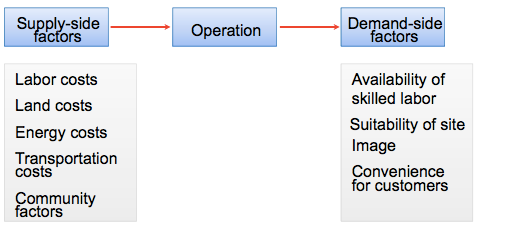
\includegraphics[width=1\textwidth]{W05/locationofoperations}
\subsubsection{Example: Cost Breakdown of Shirt Produced in Various Countries and Sold in France}
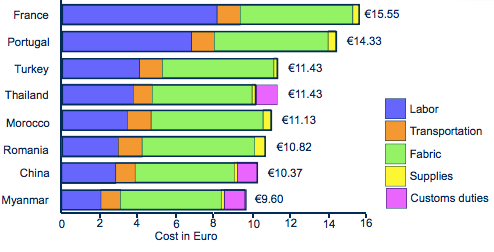
\includegraphics[width=1\textwidth]{W05/transportcost}
\subsection{Basic Layout Design\index{Layout!Design}\index{Layout}}
\subsubsection{Process Design: Design Procedure}
\index{Process!Design}
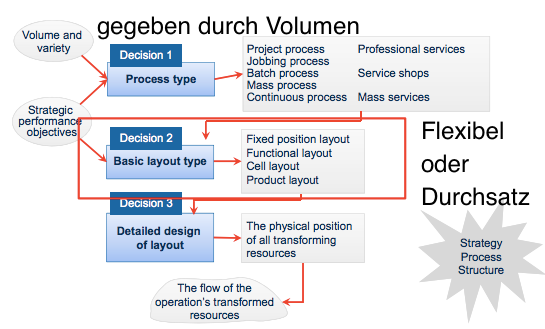
\includegraphics[width=1\textwidth]{W05/designrocess}
\subsubsection{The Nature of the Basic Layout Types}
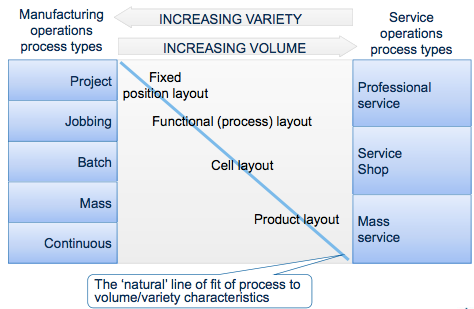
\includegraphics[width=1\textwidth]{W05/basiclayouttypes}
\subsubsection{Example of a Fixed Position Layout\index{Fixed Position Layout}: Hotel Construction Site}
Festplatz, Werft, Flugzeugbau
\begin{itemize}
\item kann nicht bewegt werden 
\item Kostenintensiv
\item Robust
\item Fixpreis -> immer mit konkretem Plan
\end{itemize}
\subsubsection{Example of  Fixed Position Layout\index{Fixed Position Layout}: Hospital OR}
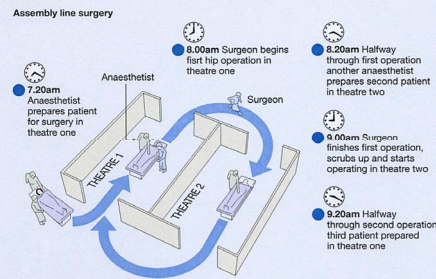
\includegraphics[width=1\textwidth]{W05/assemblylinesurgery}
\subsubsection{Example of Functional Layout\index{Functional Layout}: Glassblowing Workshop}
\subsubsection{Example of Functional Layout\index{Functional Layout}: Machine Construction}
F\"ahigkeiten werden zusammengezogen. Jegliches Produkt kann hergestellt werden. Engpass nicht Sichtbar. Lange Durchlaufszeiten.\\
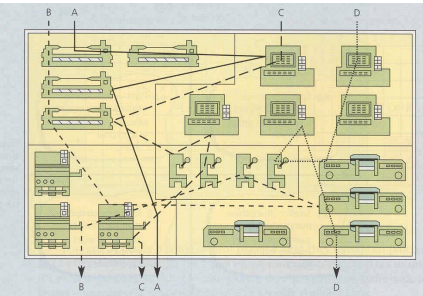
\includegraphics[width=1\textwidth]{W05/machineconstruction}
\subsubsection{Example of Functional Layout\index{Functional Layout} : Library Floor Plan}
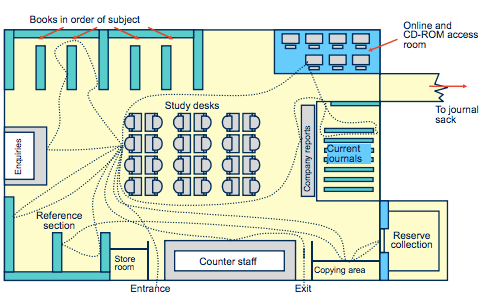
\includegraphics[width=1\textwidth]{W05/libraryfloorplan}
\subsubsection{Example of Functional Layout\index{Functional Layout} (Process): Kitchen}
\subsubsection{Example of Cell Layout\index{Cell Layout}: Machine Construction}
Flexiblit\"at nimmt ab. 5. Zelle als Werkstatt (Prototypen \& Lehrlinge). Volumen muss hoch sein. Sonst entsteht viel Leerlauf.\\
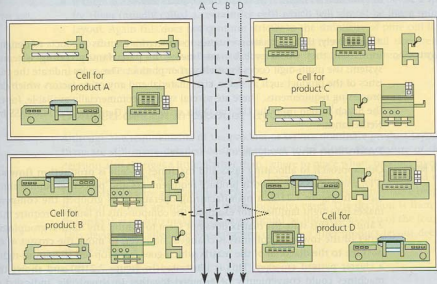
\includegraphics[width=1\textwidth]{W05/celllayoutmachine}
\subsubsection{Example of Cell Layout\index{Cell Layout}: Pharmaceutical Production}
\subsubsection{Example of Cell Layout\index{Cell Layout}: Department Store Floor Plan}
Service kann gezielt bezogen werden. Achtung, mit zentraler Kasse kein Cell Layout mehr.\\
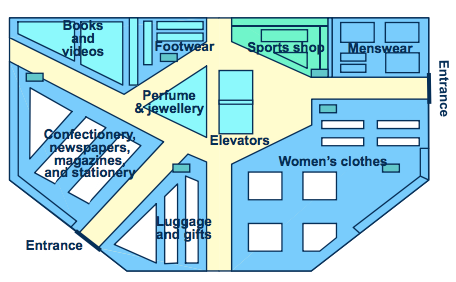
\includegraphics[width=1\textwidth]{W05/departementstore}
\subsubsection{Example of Product Layout\index{Product Layout}: Paper Production}
\subsubsection{Example of Product Layout\index{Product Layout}: Airport}
\subsubsection{Example of Product Layout\index{Product Layout}: Army Induction Center}
\subsubsection{Restaurant Using All Four Basic Layout\index{Basic Layout} Types}\label{allLayouts}
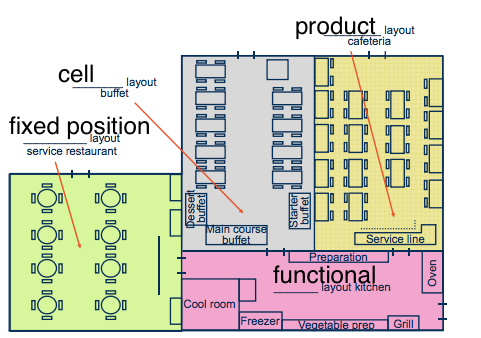
\includegraphics[width=1\textwidth]{W05/alllayouts}
\subsubsection{Revision: Basic Layout\index{Basic Layout} Types}
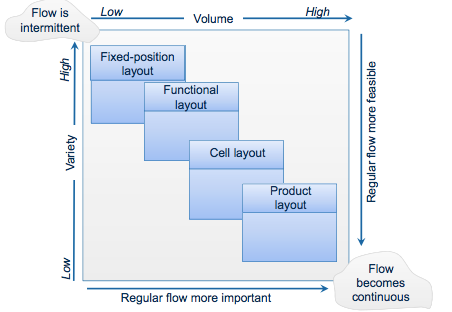
\includegraphics[width=1\textwidth]{W05/basiclayouttypesrevision}
\subsubsection{Advantages and Disadvantages}
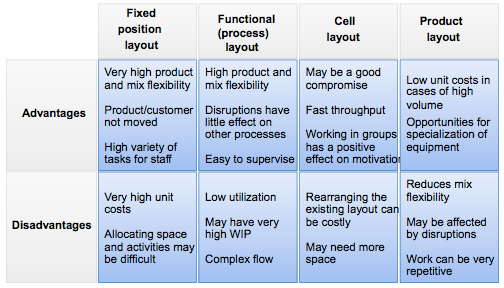
\includegraphics[width=1\textwidth]{W05/advantagesanddisadvantages}
\subsubsection{The Different Fixed and Variable Cost Characteristics Determine the Choice of Layout Type}
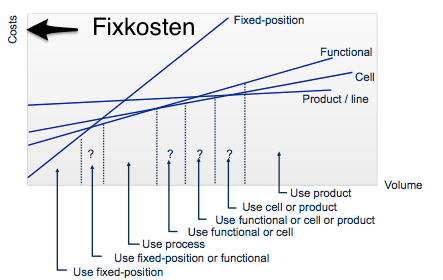
\includegraphics[width=1\textwidth]{W05/choicelayouttype}
\subsubsection{The Right Layout Type Is One Lever in Leveraging the Learning Curve}
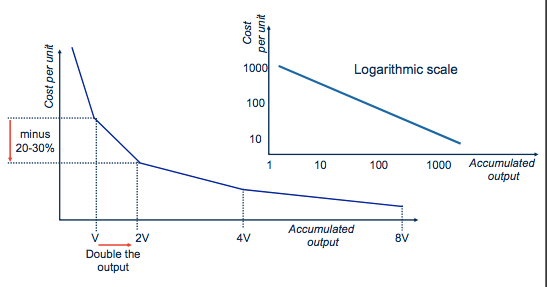
\includegraphics[width=1\textwidth]{W05/learningcurve}
\subsubsection{Examples of Learning Curve Slopes}
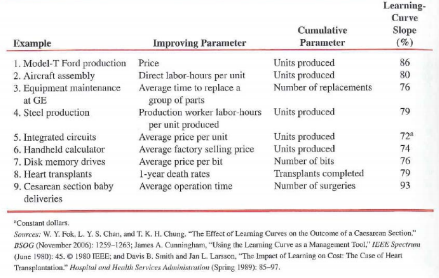
\includegraphics[width=1\textwidth]{W05/learningcourveslope}
\subsection{Workplace Design}
\subsubsection{The objectives of job design}
\subsubsection{Is Your Mouse Making You Ill?}
\subsubsection{Definition Ergonomics}
\subsubsection{Ergonomics: Legal Requirements}
\subsubsection{Ergonomics – How an Individual Interfaces with the Physical Aspects of His or Her Workplace}
\subsubsection{Job Design – Your Job as Manager Is to Define the Right Ergonomics for Your Team}
\begin{itemize}
\item Eliminate health riskis
\item Reduce health risks
\item Provide protection
\end{itemize}
\subsubsection{Group Exercises at the Conveyor Belt to Improve Health and Fight Burnout}
\subsubsection{Usability Engineering (Software Ergonomics)}
\subsubsection{Usability is key for a positive user experience}
\subsubsection{Basic Principles of Usability Engineering}
\subsubsection{What Is my function in an app?}
\subsubsection{Basic Principles of Usability Engineering}
\subsubsection{Usability Engineering (Software Ergonomics)}
